\begin{landscape}
\begin{figure}[!ht]
\begin{center}
  \begin{subfigure}{\textwidth}
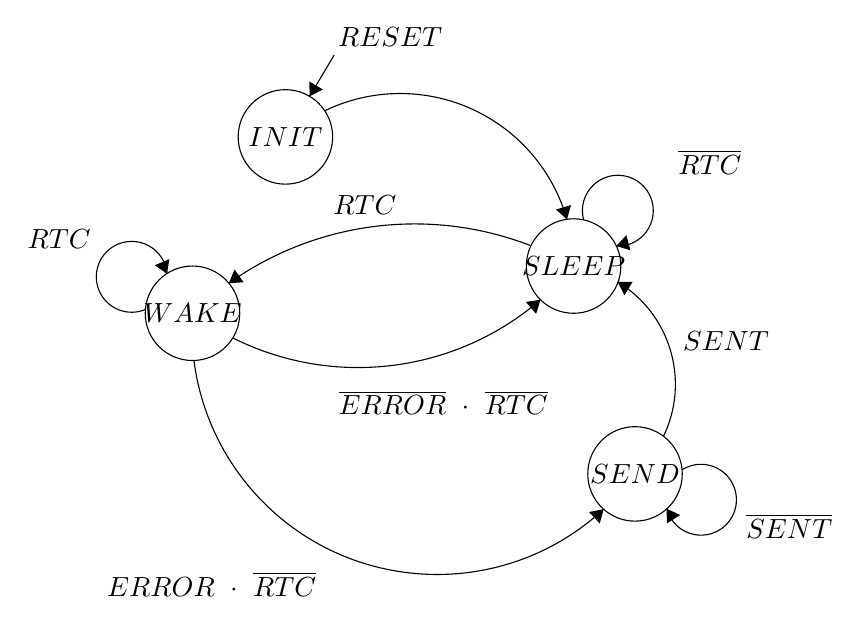
\begin{tikzpicture}[scale=0.2]
\tikzstyle{every node}+=[inner sep=0pt]
\draw [black] (36.8,-8) circle (3);
\draw (36.8,-8) node {$INIT$};
\draw [black] (55.1,-16.2) circle (3);
\draw (55.1,-16.2) node {$SLEEP$};
\draw [black] (30.9,-19.2) circle (3);
\draw (30.9,-19.2) node {$WAKE$};
\draw [black] (59,-29.4) circle (3);
\draw (59,-29.4) node {$SEND$};
\draw [black] (39.9,-2.8) -- (38.34,-5.42);
\draw (43.45,-2.3) node [above] {$RESET$};
\fill [black] (38.34,-5.42) -- (39.18,-4.99) -- (38.32,-4.48);
\draw [black] (39.29,-6.344) arc (115.82686:15.90003:11.012);
\fill [black] (54.68,-13.24) -- (54.94,-12.33) -- (53.98,-12.61);
\draw [black] (55.741,-13.281) arc (195.34019:-92.65981:2.25);
\draw (63.76,-10.43) node [above] {$\overline{RTC}$};
\fill [black] (57.81,-14.93) -- (58.71,-15.2) -- (58.45,-14.24);
\draw [black] (33.209,-17.289) arc (125.38493:68.74853:20.376);
\fill [black] (33.21,-17.29) -- (34.15,-17.23) -- (33.57,-16.42);
\draw (41.85,-12.97) node [above] {$RTC$};
\draw [black] (57.903,-17.214) arc (58.79222:-25.87219:7.596);
\fill [black] (57.9,-17.21) -- (58.33,-18.06) -- (58.85,-17.2);
\draw (62.02,-20.97) node [right] {$SENT$};
\draw [black] (53.003,-18.341) arc (-49.24761:-116.61893:17.757);
\fill [black] (53,-18.34) -- (52.07,-18.48) -- (52.72,-19.24);
\draw (46.82,-24.07) node [below] {$\overline{ERROR}\mbox{ }\cdot\mbox{ }\overline{RTC}$};
\draw [black] (57.009,-31.638) arc (-47.17822:-172.72249:15.564);
\fill [black] (57.01,-31.64) -- (56.08,-31.82) -- (56.76,-32.55);
\draw (32.12,-35.61) node [below] {$ERROR\mbox{ }\cdot\mbox{ }\overline{RTC}$};
\draw [black] (61.977,-29.145) arc (122.62938:-165.37062:2.25);
\draw (66.04,-32.72) node [right] {$\overline{SENT}$};
\fill [black] (61.01,-31.61) -- (61.02,-32.55) -- (61.87,-32.01);
\draw [black] (27.922,-18.955) arc (293.03624:5.03624:2.25);
\draw (24.47,-14.46) node [left] {$RTC$};
\fill [black] (29.28,-16.69) -- (29.43,-15.76) -- (28.51,-16.15);
\end{tikzpicture}
\caption{Sub Unit Functional State Diagram}
\label{fig:sub-unit-fsd-diagram}
  \end{subfigure}
  \begin{subfigure}[b]{0.5\textwidth}
      \begin{tabular}{c|cccc}
        STATE&\multicolumn{3}{c}{OUTPUTS}\\
        \hline
        &&&\\
        INIT&$RESET$&$\overline{RTC}$&$\overline{SENT}$&$\overline{ERROR}$\\
        SLEEP&$\overline{RESET}$&$\overline{RTC}$&$\overline{SENT}$&$\overline{ERROR}$\\
        WAKE&$\overline{RESET}$&$RTC$&$\overline{SENT}$&$\overline{ERROR}$\\
        SEND&$\overline{RESET}$&$\overline{RTC}$&$\overline{SENT}$&$ERROR$\\
      \end{tabular}
      \caption{Sub Unit Functional State Diagram: State and Outputs}
      \label{fig:sub-unit-fsd-state-outputs}
  \end{subfigure}
  \begin{subfigure}[b]{0.5\textwidth}
   \begin{tabular}{|c|}
    \hline
     Output List\\
    \hline
     RESET = Power on Reset\\
     SLEEP = MCU is in LPM4\\
     WAKE = RTC Timer turned on MCU\\
     SEND = Bluetooth module is sending data\\
     ERROR = Temperature or Age Related Error Detected\\
    \hline
   \end{tabular}
      \caption{Sub Unit Functional State Diagram: Output List}
      \label{fig:sub-unit-fsd-outputs-list}
  \end{subfigure}
\caption{Sub Unit Functional State Diagram}
\label{fig:sub-unit-fsd}
\end{center}
\end{figure}
